One of Dr. Jonas' greatest discoveries was the Heyting people, a democratic collection of 6 tribes that lived on the Eurasian steppes.
They kept meticulous records of their elections and their rulers.
Strangely, even though the Heyting people were democratic, the voting records indicated that many of their leaders recived far less than the majority of the votes.
How could this happen?
Each tribe elected its own ruler, and then the council of 6 rulers would meet to make decisions.
To simplify the voting process, the tribes had broke their land up into provinces, each of which would cast one vote for the next ruler of that tribe.
To figure out which vote to cast, each province would take the majority vote of its people.
To cap it off, the tribe leaders were allowed to redraw the boundaries of the provinces using the following guidelines:
\begin{enumerate}
\item The number of provinces had to stay the same.
\item No province's population could exceed any others by more than 5 people.
\item All province boundary lines had to follow the grid lines provided.
\item Given two locations in the same province, you had to be able to walk between them without crossing into any other provinces.
\end{enumerate}

Altough she was unable to find records detailing the number of provinces or their boundaries, Dr. Jonas did find records detailing a three year election cycle from each of the six tribes.
The first is shown below, with possible province boundaries drawn in by Dr. Jonas.
Notice that X won all three years even though they never had the majority vote.

Tribe A
Population = 50

\begin{tabular}{c c c }

Year 1 & Year 2 & Year 3 \\
 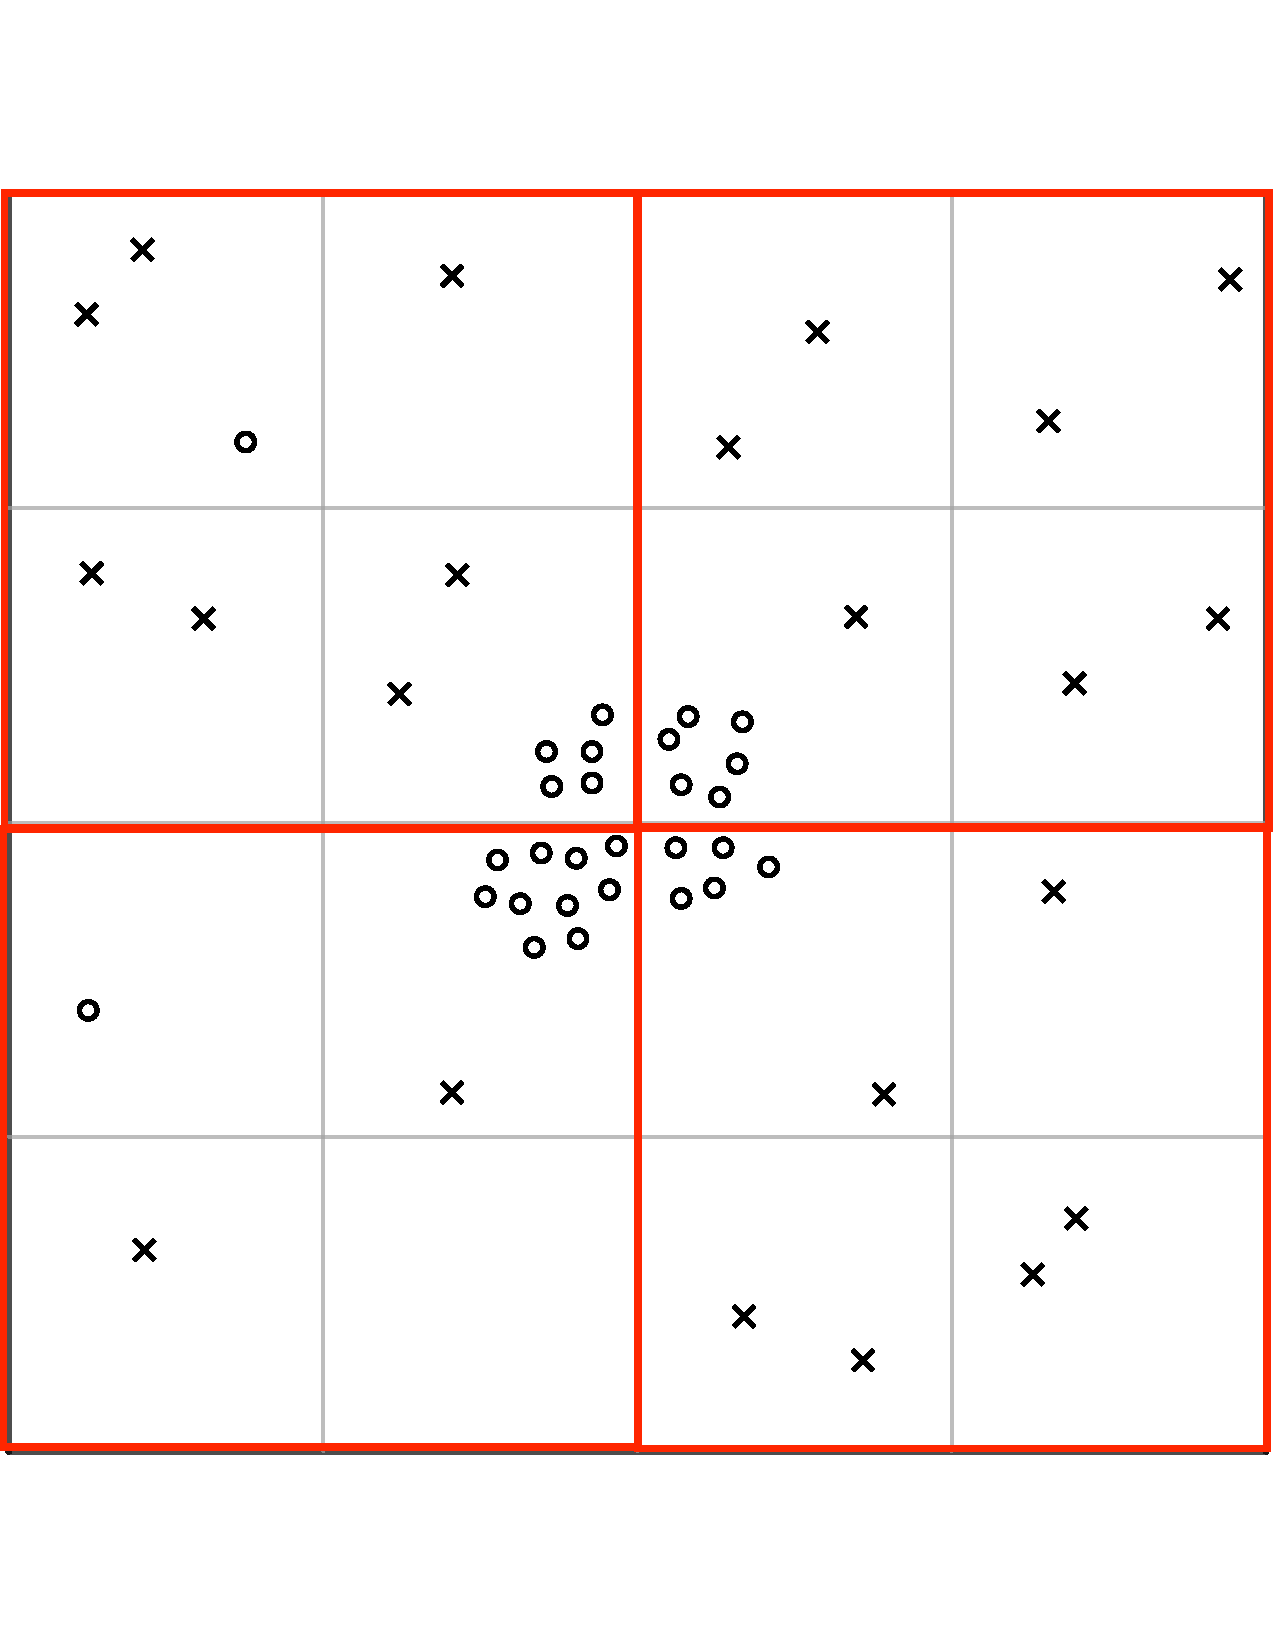
\includegraphics[width=2in]{assets/Gerrymandering/Gerry4x4-50-1Solution.pdf} &  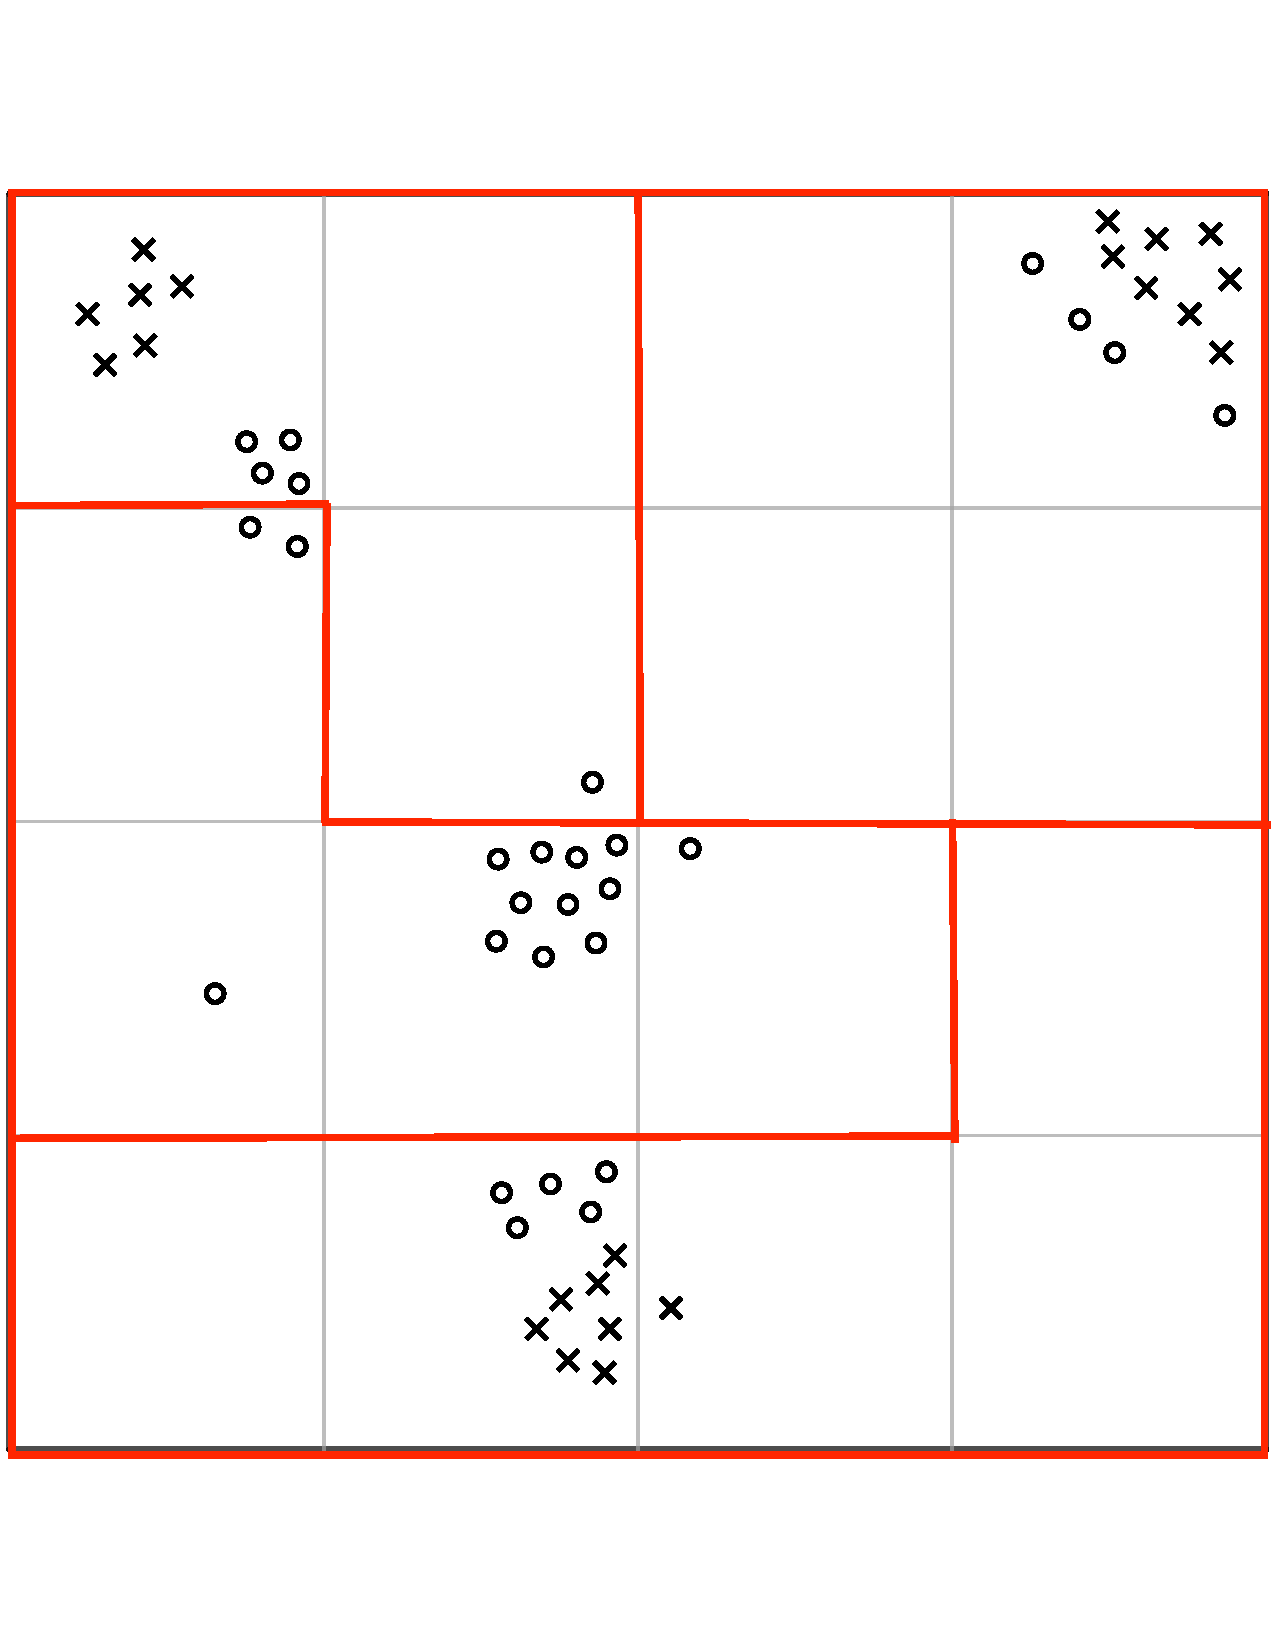
\includegraphics[width=2in]{assets/Gerrymandering/Gerry4x4-50-2Solution.pdf} &  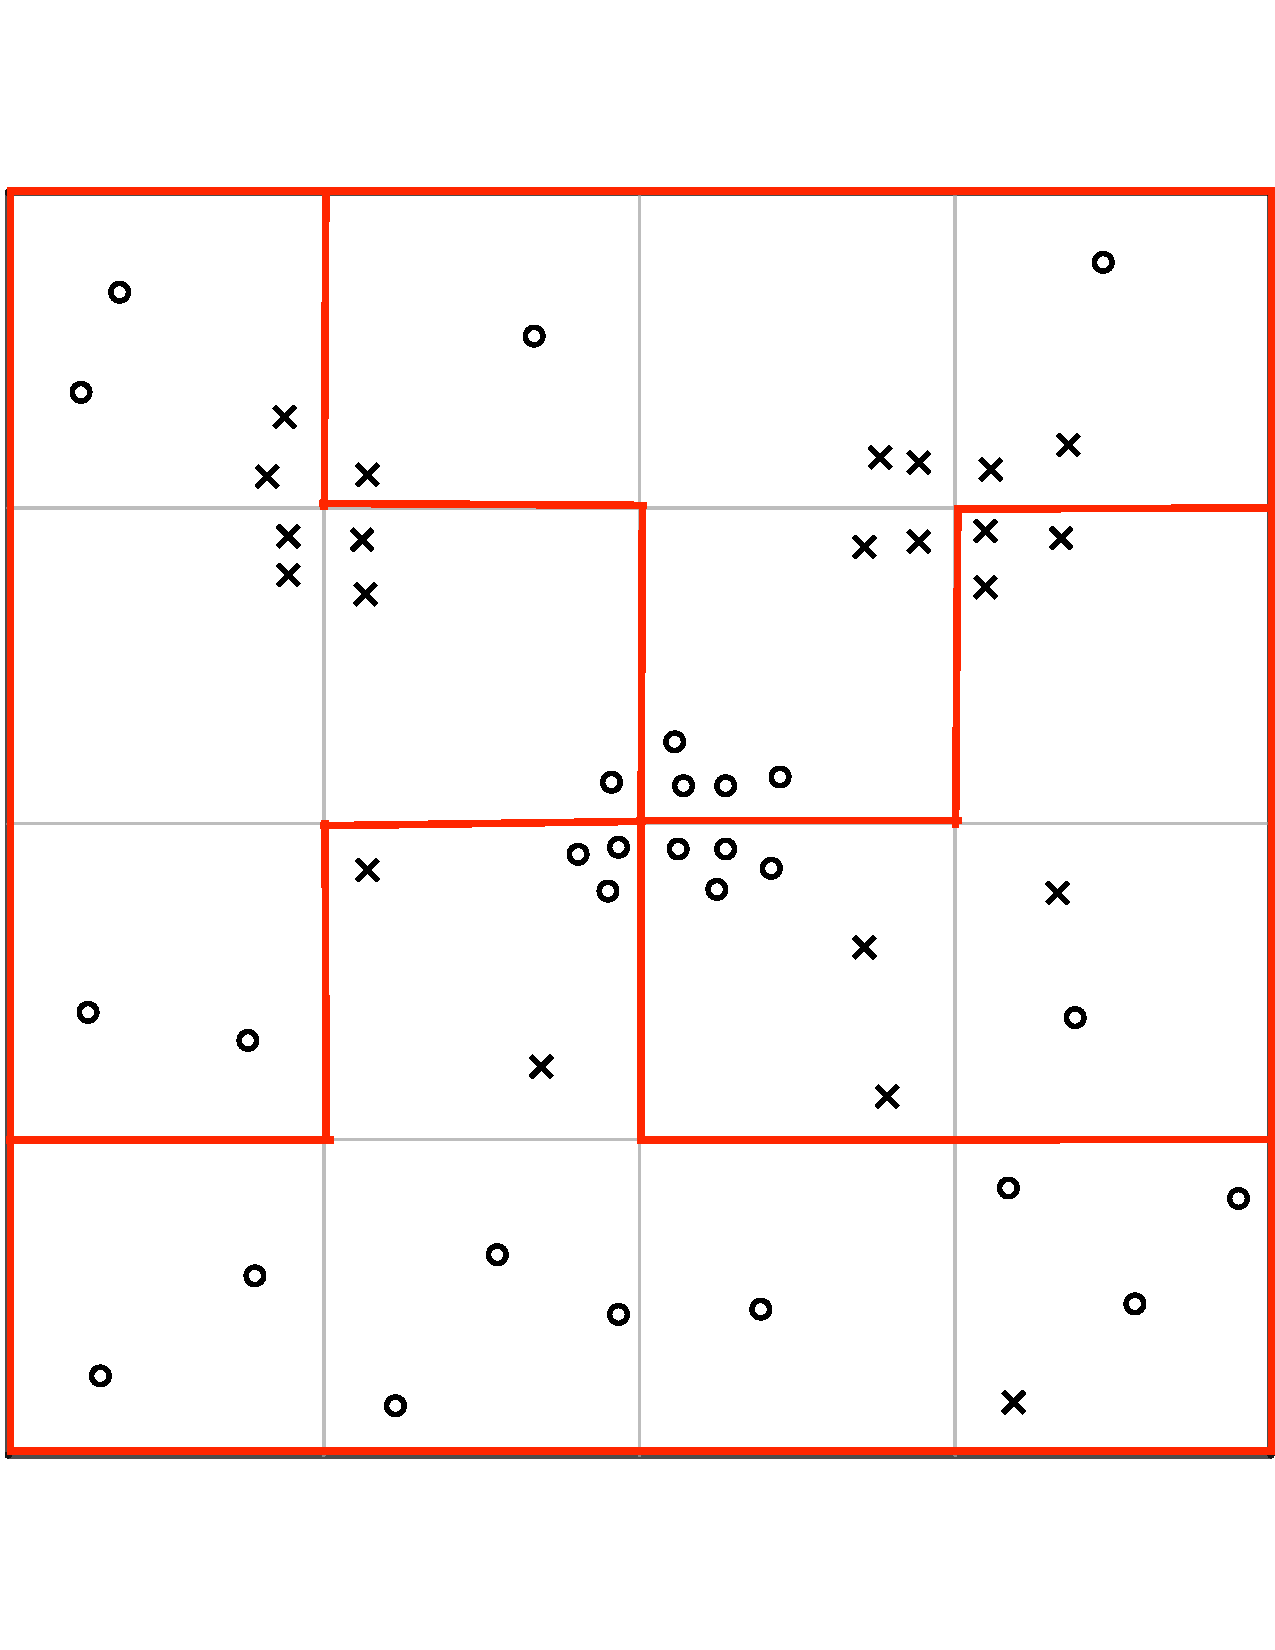
\includegraphics[width=2in]{assets/Gerrymandering/Gerry4x4-50-3Solution.pdf}\\
 Total Vote Count &  Total Vote Count &  Total Vote Count\\
 X - 22 & X - 22 & X  - 22\\
 O - 28 & O - 28 & O - 28
\end{tabular}

Dr. Jonas reasoned that there were 3 provinces for tribe A.
After finding the number of provinces for the other tribes, you should be able to decode the message in Dr. Jonas' journal.
